\documentclass[article,a4paper,oneside,10pt]{memoir}

% -------------------------------------------------------------------------- %
% Page Layout                                                                %
% -------------------------------------------------------------------------- %
\setlrmarginsandblock{0.142857111\paperwidth}{0.142857111\paperwidth}{*}
\setulmarginsandblock{0.111111111\paperheight}{*}{1.25}
\checkandfixthelayout
\newfixedcaption{\figcaption}{figure}
\newfixedcaption{\tabcaption}{table}
\captiontitlefont{\small}
\captionnamefont{\bfseries\small}
\captiondelim{: }

% -------------------------------------------------------------------------- %
% Bibliography                                                               %
% -------------------------------------------------------------------------- %
\renewcommand{\bibsection}{%
    \chapter{References}%
    \prebibhook}
\bibintoc
\renewcommand{\cftdot}{\textcolor{gray}{.}}
\renewcommand{\cftchapterdotsep}{\cftdotsep} % Chapters have dots in ToC
\renewcommand{\cftsectiondotsep}{\cftnodots} % Sections have no dots in ToC


% -------------------------------------------------------------------------- %
% Chapter and Section Headings                                               %
% -------------------------------------------------------------------------- %
\makeatletter
\makechapterstyle{alpensec}{%
  \chapterstyle{default}
  \setlength{\beforechapskip}{3.5ex \@plus 1ex \@minus .2ex}
  \renewcommand*{\chapterheadstart}{\vspace{\beforechapskip}}
  \setlength{\afterchapskip}{2.3ex \@plus .2ex}
  \renewcommand{\printchaptername}{}
  \renewcommand{\chapternamenum}{}
  \renewcommand{\chaptitlefont}{\sffamily\LARGE\bfseries}
  \renewcommand{\chapnumfont}{\chaptitlefont}
  \renewcommand{\printchapternum}{\chapnumfont \thechapter\quad}
  \renewcommand{\afterchapternum}{}}

\renewcommand{\section}{%
  \sechook%
  \@startsection{section}{1}%  level 1
      {\secindent}%            heading indent
      {\beforesecskip}%        skip before the heading
      {\aftersecskip}%         skip after the heading
      {\sffamily\secheadstyle}} % font

\makeatother

\chapterstyle{alpensec}


% -------------------------------------------------------------------------- %
% Packages                                                                   %
% -------------------------------------------------------------------------- %
\usepackage[%
        bookmarksnumbered=true,
        colorlinks=true,
        linkcolor=cyan!50!blue,
        citecolor=violet,
        urlcolor=purple,
    ]{hyperref}
\usepackage[light,nott]{kpfonts}
\usepackage{microtype}
\usepackage[english]{babel}
\usepackage[T1]{fontenc}
\usepackage[utf8]{inputenc}
\usepackage{xcolor-solarized}
\usepackage{lipsum}
\usepackage{graphicx}
% -------------------------------------------------------- %
% Minted defines the listing  environment via the newfloat %
% package. This leads to  the listoflistings being typeset %
% on the  section level,  with the entries  being indented %
% too far.  We therefore create our own listings float and %
% corresponding listof before loading minted.              %
%                                                          %
% See:                                                     %
% memman.pdf page 170                                      %
% https://github.com/gpoore/minted/issues/67               %
% -------------------------------------------------------- %
\newcommand{\listingname}{Listing}
\newcommand{\listlistingname}{List of Listings}
\newlistof{listoflistings}{lol}{\listlistingname}
\newfloat{listing}{lol}{\listingname}
\newlistentry{listing}{lol}{0}
\usepackage{minted}
\usepackage{tcolorbox}
\renewcommand{\listingscaption}{\small\bfseries Listing}


% -------------------------------------------------------------------------- %
% Macros and Config                                                          %
% -------------------------------------------------------------------------- %
\newcommand\code[1]{\texttt{#1}}
\newcommand\pacname[1]{\texttt{#1}}

\DeclareTextFontCommand{\emphc}{\color{solarized-red}\em}

\tcbuselibrary{minted}
\tcbset{
    listing and text,
    listing engine=minted,
    %title=\textsf{\bfseries Code \hfill \LaTeX{} Output},
    minted language=text,
    minted options={autogobble}}

% -------------------------------------------------------------------------- %
% Title                                                                      %
% -------------------------------------------------------------------------- %
\title{\textsf{\Huge  The Black Magic of Floats in \LaTeX}}
\author{Raphael Frey\\[2mm]\small%
    \href{https://github.com/alpenwasser/TeX/tree/master/floats}
         {\nolinkurl{https://github.com/alpenwasser/TeX/}}}

\date{\vspace{1em}\today}

% ************************************************************************** %
\begin{document}
% ************************************************************************** %


\maketitle

\vfill
\begin{abstract}
    The behavior  of floats can  often be  confusing for the  uninitiated, and
    yield  unexpected results. This  document gives  a brief  overview on  the
    subject, primarily based on Leslie  Lamport's \emph{\LaTeX{} -- A Document
    Preparation System} \cite{lamport}.

    This document does  not cover every possible edge case,  but presents some
    usage examples and common problem one tends to run into while working with
    floats.   It also  presents  some  alternatives for  when  floats may  not
    necessarily be the most sensible solution.
\end{abstract}

\vfill
\tableofcontents*
\vfill
\newpage
\listoflistings*
\label{lol}
\listoffigures*
\listoftables*


% ========================================================================== %
\newpage
\chapter{Incomplete Summary for the Impatient}
\label{chap:summary}
% ========================================================================== %

\vfill
\begin{tcblisting}{%
        title={\bfseries\sffamily Default Float Environments in \LaTeX},
        comment={%
            The starred  versions produce  double-column floats  in two-column
            documents.   They are  identical  to the  non-starred versions  in
            single-column documents.  See Section~\ref{chap:placement} on 
            page~\pageref{chap:placement} for the meaning of \code{loc}.},
        listing and comment,
        minted language=tex,
        minted options={autogobble,escapeinside=||}}
        \begin{figure}[loc]   body   \end{figure}
        \begin{figure*}[loc]  body   \end{figure*}
        \begin{table}[loc]    body   \end{figure}
        \begin{table*}[loc]   body   \end{figure*}
\end{tcblisting}

\vfill
\begin{tcblisting}{%
        title={\bfseries\sffamily Example: Table, Centered, Labeled and Captioned},
        comment={%
            Note  that  the  \code{\textbackslash   label}  must  come  either
            inside  or after  the  \code{\textbackslash caption}  command. For
            \code{figure}s,  the  caption  and  label are  usually  below  the
            content, for \code{table}s above.},
        listing and comment,
        minted language=tex,
        minted options={autogobble,escapeinside=||}}
        \begin{table}
            \centering
            \caption{A table of curiosities}
            \label{tab:cur-table}
            \begin{tabular}{ll}
                \scshape Observation              & \scshape Explanation      \\
                Sun rose in the west this morning & universe is broken, or:   \\
                                                  & too many drugs            \\
                rain is falling upwards           & definitely too many drugs \\
            \end{tabular}
        \end{table}
\end{tcblisting}

\vfill
\begin{tcblisting}{%
        title={\bfseries\sffamily Print Leftover Floats},
        comment={%
            The  \code{\textbackslash clearpage}  command prints  any leftover
            floats, putting them on separate  pages with no text. It is useful
            for ensuring  that no floats from  one chapter are printed  on the
            first page(s) of a new chapter.
            
            In    \code{twoside}     documents,    the    \code{\textbackslash
            cleardoblepage} command can  be used to ensure that  a new section
            is only started on a right-hand page.

            Multiple commands will not produce multiple empty pages.},
        listing and comment,
        minted language=tex,
        minted options={autogobble,escapeinside=||}}
        \clearpage
        \cleardoublepage
\end{tcblisting}

\vfill
Some packages which might be of interest when working with floats, for example
for  customizing  captions,  creating  new captions  and  creating  new  float
environments, can  be found  the Bibliography  on page~\pageref{bibliography}.
Specifically the packages
\pacname{caption}~\cite{ctan:package:caption},
\pacname{floatrow}~\cite{ctan:package:floatrow},
\pacname{float}~\cite{ctan:package:float},
\pacname{capt-of}~\cite{ctan:package:capt-of},
and \pacname{captdef}~\cite{ctan:package:captdef}.


% ========================================================================== %
\newpage
\chapter{What Are Floats, Anyway?}
\label{chap:what-are-floats}
% ========================================================================== %

Normal text  is broken  by \TeX{} across  lines and  pages automatically. Some
content, such as images, are not  well-suited to being split into pieces. That
is what floating environments are for: To provide a way to put such content in
a  place  where  it does  not  need  to  be  broken;  a mechanism  for  it  to
\emph{float} to a suitable location for an optimal overall result.

Two  such  floating environments  are  provided  by \LaTeX{}  by  default: The
\verb|figure|   and  the   \verb|table|\footnotemark  environment. There   are
packages   which  define   more  floating   environments  (for   example,  the
\verb|listings| packages can  let its code listings float, if  so desired), or
the user may define their own floating environments, if they so wish.

\footnotetext{%
    Because confusion is fun: The \texttt{table} environment does not actually
    typeset  a table.   That is  what \texttt{tabular},  \texttt{tabularx} and
    similar environments are for. See  \cite{mori:tables} for an overview. The
    \texttt{table}  environment is  merely a  floating container  intended for
    containing tabular content.}

Fundamentally, the only important difference between these environments is how
they are  captioned and numbered:  \verb|figure| environments get  a different
caption  and  number  than  \verb|table|  environments. However,  one  may  in
principle put  pretty much  anything one  desires into  either environment. As
long  as  the  code  itself  is  valid,  \LaTeX{}  will  not  complain. Figure
\ref{fig:lipsum} demonstrates this by placing some Lorem Ipsum text inside its
environments.

The floating behavior can be demonstrated by the fact that, in the source code
of this  document, Figure \ref{fig:lipsum} and  Table \ref{tab:experiment} are
placed almost right  after this sentence. In the resulting  document, they may
be placed  wherever \LaTeX{}  deems most  suitable\footnotemark.

\footnotetext{%
    \LaTeX{} usually tries  to place floats either  at the top of  a page, the
    bottom of a page, or  on a separate page. See Section~\ref{chap:placement}
    for more information.}


\begin{figure}
    {\color{gray}\centering\small\lipsum[1]}
    \caption{A \texttt{figure} environment with placeholder text}
    \label{fig:lipsum}
\end{figure}

\begin{table}
    \centering
    \caption{Results for an experiment}
    \label{tab:experiment}
    \begin{tabular}{ll}
        \toprule
        \scshape Experiment Input & \scshape Experiment Output \\
        \midrule
        interesting thing         & interesting result!        \\
        boring thing              & mildly surprising result   \\
        weird thing               & very unexpected result     \\
        fascinating thing         & machine broke              \\
        Xenomorph XX121           & dead scientists            \\
        \bottomrule
    \end{tabular}
\end{table}


% ========================================================================== %
\chapter{Basic Usage}
\label{chap:basic-usage}
% ========================================================================== %


Listing \ref{lst:figure}\footnotemark  shows the  basic code for  including an
external  graphics file  inside a  \verb|figure| environment  and providing  a
caption and label to go along with it.

\footnotetext{%
    Incidentally, Listing \ref{lst:figure}  is one of those cases  where a new
    type  of floating  environment  has been  provided; in  this  case by  the
    \texttt{minted} package.}

\begin{listing}
    \begin{tcblisting}{%
            title={\bfseries\sffamily Figure Environment with External Picture},
            minted language=tex,
            listing only,
            minted options={autogobble,escapeinside=||}}
        \begin{figure}
            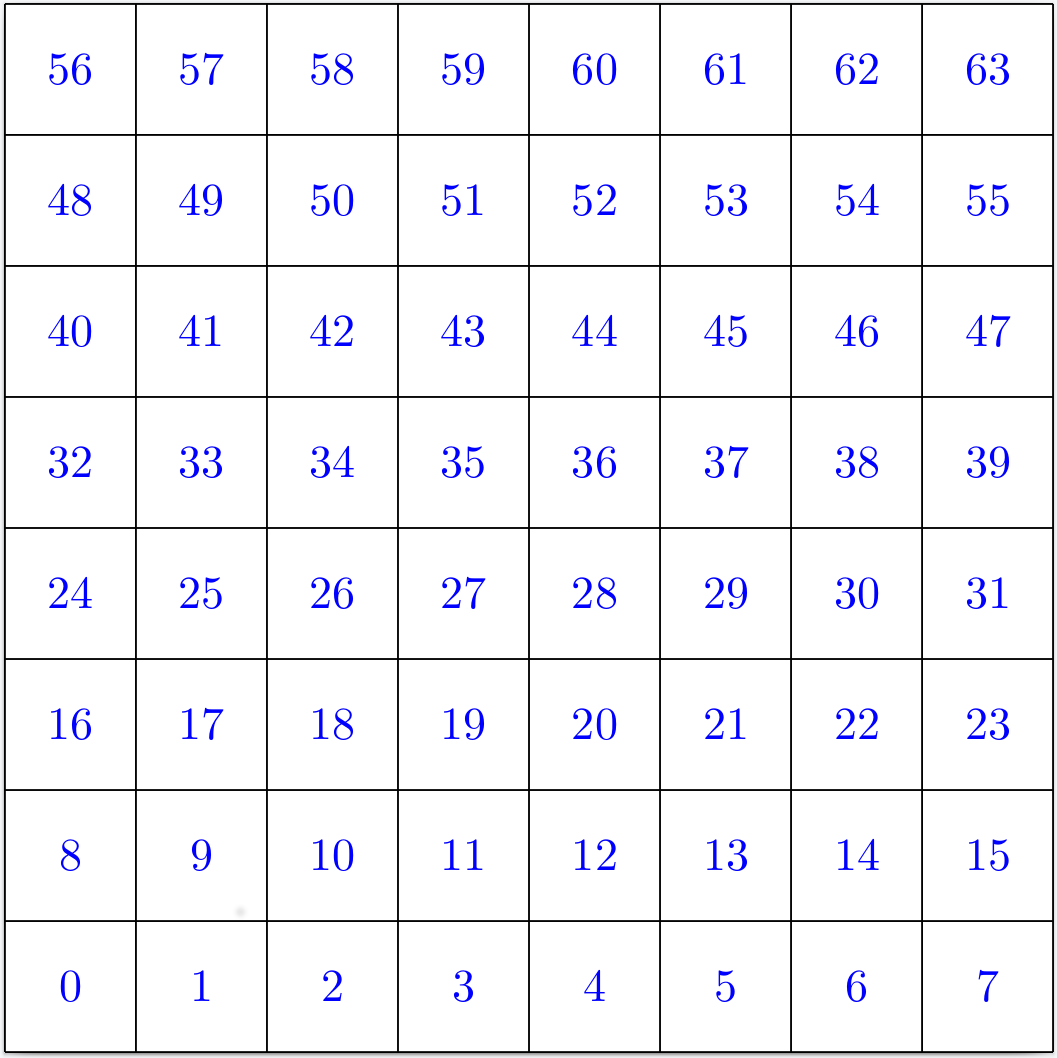
\includegraphics[height=3cm,width=4.5cm]{images/grid8cm.png}
            \caption{This is a distorted grid.}
            \label{fig:distorted-grid}
        \end{figure}
    \end{tcblisting}
    \caption{%
        Code block for  including a graphics in a figure  and adding a caption
        and  a label  so that  we can  refer to  the figure  elsewhere in  the
        text. Note  that the  \code{\textbackslash  label}  command must  come
        either inside or after the \code{\textbackslash caption} command.}
    \label{lst:figure}
\end{listing}


It is  often desirable to center  a table or a  picture, in which case  we add
a  \verb|\centering|  directive  into  the environment,  as  done  in  Listing
\ref{lst:centering}\footnotemark.

\footnotetext{%
    There     exists     also    a     \texttt{\textbackslash{}begin\{center\}
    \ldots   \textbackslash{}end\{center\}}   environment. For  the   curious,
    some    information    on    the     differences    between    that    and
    \texttt{\textbackslash{}centering} can be found at
    \cite{stackexch:center-centering,texblog:center-centering}}

\begin{listing}
    % ---------------------------------------------------- %
    % Note that  we have to  do a bit of  workaround magic %
    % inside the  escaped part  of the  minted environment %
    % because it drops us back into LaTeX.                 %
    % ---------------------------------------------------- %
    \begin{tcblisting}{%
        title={\bfseries\sffamily Tabular Inside Table, Centered},
        listing only,
        minted options={autogobble,escapeinside=||}}
        \begin{table}
            |\textcolor{solarized-red}{\textbf{\textbackslash{}centering}}|
            \caption{Results for an experiment}
            \label{tab:experiment}
            \begin{tabular}{ll}
                \toprule
                \scshape Experiment Input & \scshape Experiment Output \\
                \midrule
                interesting thing         & interesting result!        \\
                boring thing              & mildly surprising result   \\
                weird thing               & very unexpected result     \\
                fascinating thing         & machine broke              \\
                Xenomorph XX121           & dead scientists            \\
                \bottomrule
            \end{tabular}
        \end{table}
    \end{tcblisting}
    \caption[Centering a Float]{%
        Centering  a  \texttt{tabular}  environment  inside  a  \texttt{table}
        floating   environment. This   is   actually  the   code   for   Table
        \ref{tab:experiment}.}
    \label{lst:centering}
\end{listing}


You may have noticed that the  \verb|\caption| is placed above the content for
tables  and below  the picture  in  a \verb|figure|  environment. This is  not
prescribed by  \LaTeX, obviously, and  will depend  on the style  guide you're
following or your own preferences. All I will  say on the subject is that most
tables I've seen  had their caption above  the table and most  images had them
below the picture.

\emph{What does matter, however,  is where the \texttt{\textbackslash{}label}
is put!} In order  to pick up the  correct number, it must  always come either
inside the  \verb|\caption| command to which  is is supposed to  be connected,
or  after  it.   If  you  put  it  before  the  \verb|\caption|  command,  the
\verb|\label| will  pick up whichever counter  was the last active  one before
the \verb|\caption|, which can be anything  (another picture or table or float
of some sort, but also a chapter, section or similar). This is a mistake which
is easily made and often hard to detect.

Also  note  the  optional  argument  to  the  \verb|\caption|  command. If  it
is  given,  it  will  be  the  text for  the  entry  in  the  \verb|listof...|
command. See Listing \ref{lst:caption-opt-arg} and the \emph{List of Listings}
on page~\pageref{lol}.


\begin{listing}
    \begin{tcblisting}{%
            title={\bfseries\sffamily%
                Optional Argument for \code{\textbackslash{}caption} Command},
            minted language=text,
            listing only,
            minted options={autogobble,escapeinside=||}}

        \caption|\textcolor{solarized-red}{[This is the text for the List of <something> entry]}|{
            This is the  text which goes below/above the  float. It can be
            rather  long, depending  on how  much explanation  the content
            of  the  float requires  (remember:  because  a float  is  not
            necessarily right  where you  write about  its content  in the
            main  body of  text,  it might  be useful  for  the reader  to
            understand its  content without having  to go and  dig through
            the main text),  and in such cases, it does  not make sense to
            have the entire text of the caption in the List of entry.}
    \end{tcblisting}
    \caption[Optional Arguments for \code{\textbackslash caption}]{%
        Optional  Argument to  the \code{\textbackslash{}caption}  command for
        the  \code{List of  \ldots} entry. You  can  see what  happens in  the
        \emph{List of Listings} when we do not use this optional argument with
        the  entry  for  Listing~\ref{lst:figure}. Compare to  the  \emph{LoL}
        entry for this listing on  page~\pageref{lol}, which is short, despite
        this rather lengty caption text.}
    \label{lst:caption-opt-arg}
\end{listing}


Lastly: Because captions  are a moving  argument (Section 2.2.3, page  22, and
Section 3.5.1, page 58 in \cite{lamport}), fragile commands such as linebreaks
inside them  must be preceded by  \verb|\protect|, as shown in  the caption of
Figure \ref{fig:protect} and the code in Listing \ref{lst:caption:linebreak}.

The \verb|\caption|  command can  only be used  inside a  floating environment
by  default  (that's  how  \verb|\caption|  knows  whether  it's  supposed  to
say  \emph{Figure  \code{n}}  or  \emph{Table  \code{m}},  for  example).   If
you   require  captions   for   non-floating  content,   there  are   packages
which  provide  such  facilities,  as   well  as  more  caption  customisation
options;   see   \cite{ctan:package:caption,ctan:topic:caption}  and   Chapter
\ref{chap:alternatives} of this document.


\begin{figure}
    \centering
    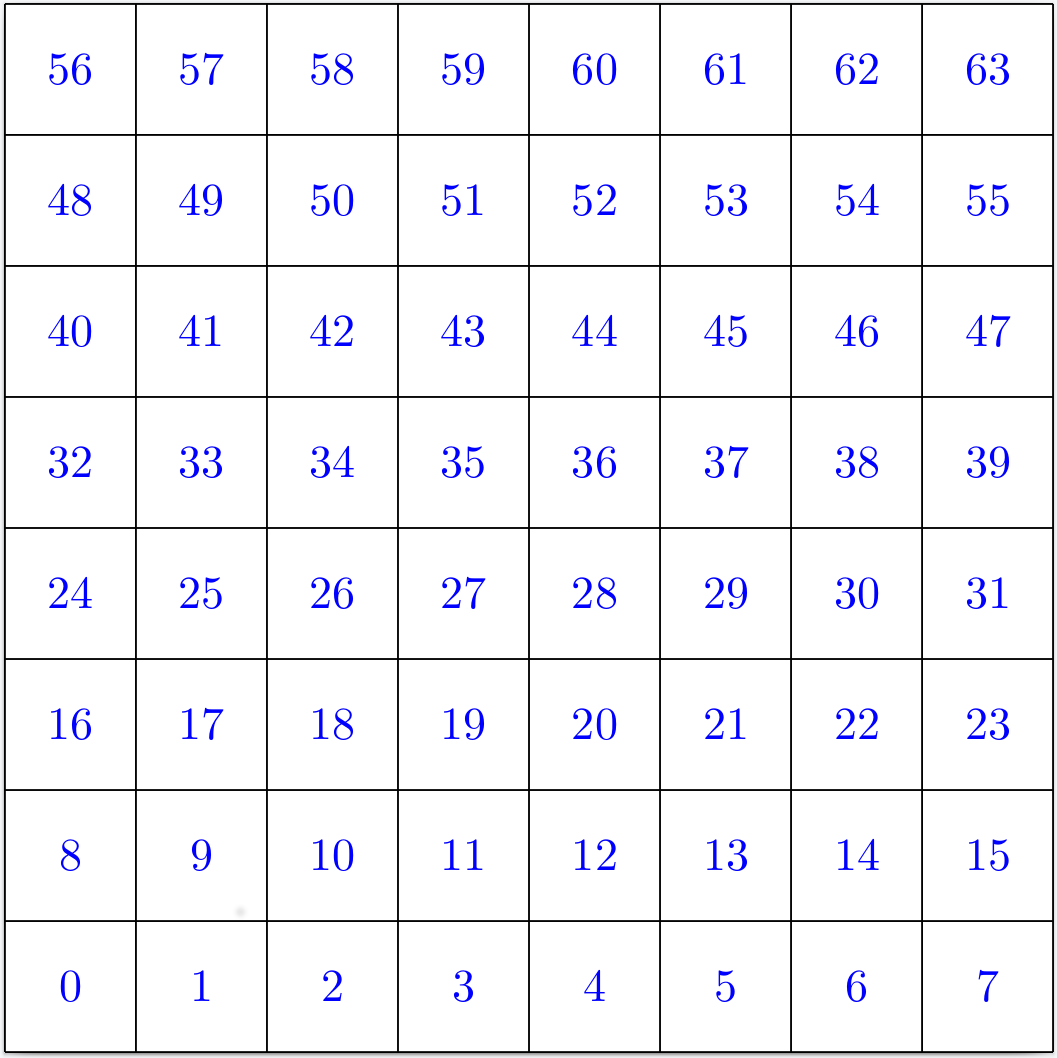
\includegraphics[height=4cm,width=4cm]{images/grid8cm.png}
    \caption[Linebreaks in Captions]{%
        A  classic use  case  of the  \code{figure}  environment: including  a
        graphics file.\protect\\
        You can also  have linebreaks inside a \code{caption},  like here, but
        it requires the \code{\textbackslash{}protect} command, and there must
        be  no empty  line after  the \code{\textbackslash\textbackslash}. See
        Listing \ref{lst:caption:linebreak} for the code.}
    \label{fig:protect}
\end{figure}

\begin{listing}
    \begin{tcblisting}{%
            title={\bfseries\sffamily Linebreaks in Captions},
            minted language=text,
            listing only,
            minted options={autogobble,escapeinside=||}}
        \begin{figure}
            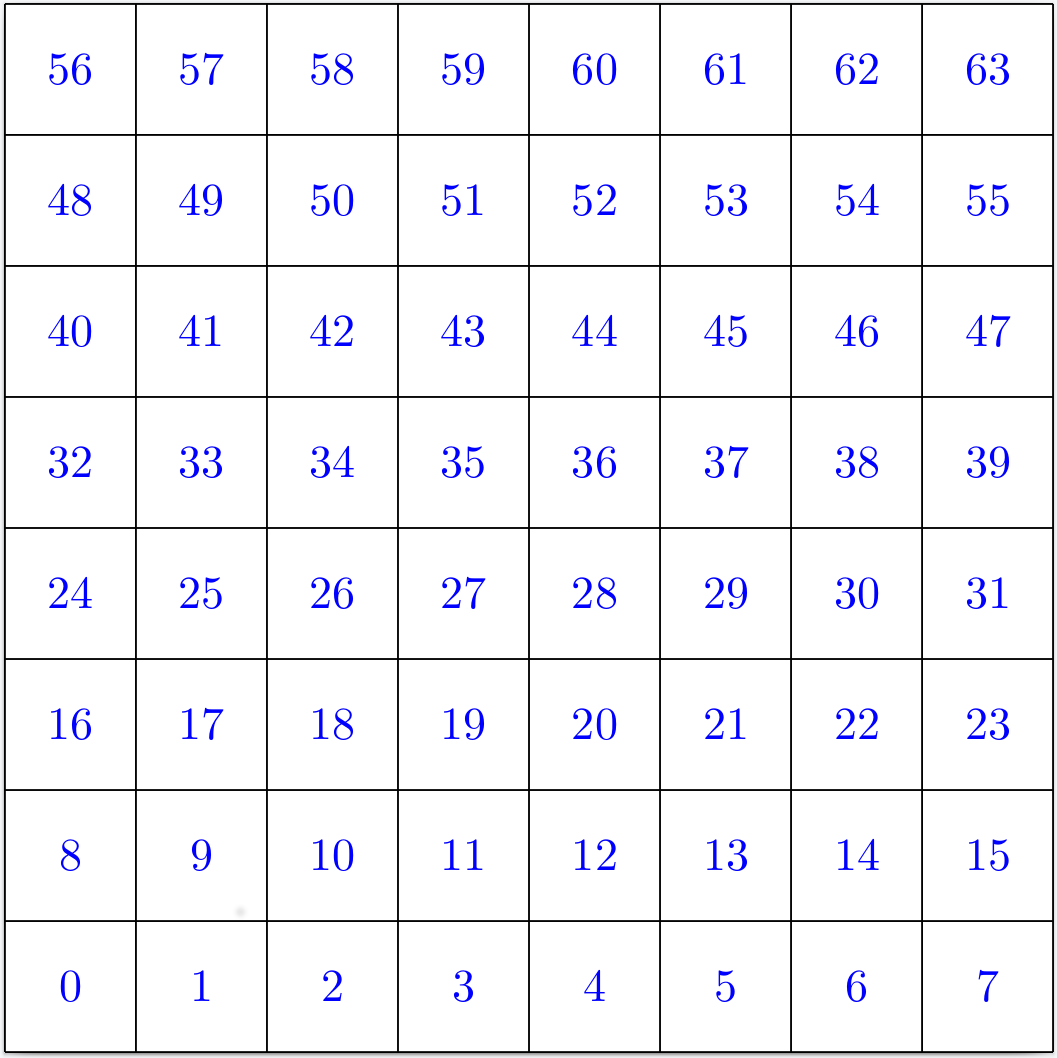
\includegraphics[height=3cm,width=4.5cm]{images/grid8cm.png}
            \caption{%
                Here we have a sentence.|\textcolor{solarized-red}{\bfseries\textbackslash{}protect\textbackslash\textbackslash}|
                And this sentence will be on a new line.}
            \label{fig:distorted-grid}
        \end{figure}
    \end{tcblisting}
    \caption{%
        Code  block for  including  a forced  linebreak in  a  caption with  a
        \code{\textbackslash{}protect} command}
    \label{lst:caption:linebreak}
\end{listing}


% ========================================================================== %
\clearpage
\chapter{Placement Options}
\label{chap:placement}
% ========================================================================== %

Placement  options  allow you  to  influence  \LaTeX's placement  behavior  of
floats, with more or less vehemence.

\emph{Whatever your preferences, only use placement options once your text is
(almost) complete!} Otherwise you will end up needing to change them again and
again and again, causing a lot more work. Also, it is quite easily possible to
overlook  a  bad placement  option  from  an  earlier  version of  a  document
which  makes  you jump  through  hoops  trying to  get  the  best result  even
though  \LaTeX{} would  actually do  the  right thing  if you  would just  let
it\footnotemark.

\footnotetext{%
    I am  obviously \emph{not}  speaking from  personal experience  here. I am
    smarter than that, I assure you.}

\begin{listing}
    \begin{tcblisting}{%
            title={\bfseries\sffamily%
                Placement Options},
            minted language=tex,
            listing only,
            minted options={autogobble,escapeinside=||}}
            \begin{float type}[|\textcolor{solarized-red}{loc}|] body \end{float type}
    \end{tcblisting}
    \caption{Placement options for floats}
    \label{lst:placement-options}
\end{listing}

Listing \ref{lst:placement-options} contains the basic  syntax of a float with
placement options. The  \code{loc} argument can be  a sequence of one  to four
letters and an exclamation mark. It specifies  where \LaTeX\ is allowed to put
the  float. The meaning  of  these  options is  as  follows (paraphrased  from
\cite{lamport}):

\begin{itemize}
    \item  [\code{\color{solarized-red}h}] \emph{Here:}  at  the  location in  the  text where  the
        environment is  in the  source code. Does  not work  for double-column
        floats in two-column documents.

    \item [\code{\color{solarized-red}t}] \emph{Top:} at the top of a text page.

    \item [\code{\color{solarized-red}b}]  \emph{Bottom:} at  the bottom of  a text  page. Does not
        work for double-column floats in two-column documents.

    \item [\code{\color{solarized-red}p}] \emph{Page of floats:} on a separate page containing only
        floats, but no text.

    \item [\code{\color{solarized-red}!}] \emph{Try harder:} tells  \LaTeX{} to try harder to place
        the float  at the earliest possible  place in the document  allowed by
        the  rest  of  the  argument. The  meaning  of  \emph{try  harder}  is
        elaborated in Section \ref{chap:innards}.

        This also  overrides a  potential \verb|\suppressfloats|  command (see
        below) for the float to which the \code{loc} argument belongs.
\end{itemize}

The  default  value for  \code{loc},  if  it  is  not specified  manually,  is
\code{tpb}, meaning \LaTeX{} may put the float  at the top of a text page, the
bottom of a text page, or on a separate page containing only floats.

When  an  optional  \code{loc}  argument   is  given,  make  sure  to  specify
enough  options to  allow  \LaTeX{} sufficient  flexibility  with placing  the
floats. Otherwise a  float and all  subsequent floats  can end up  being saved
until the end of a chapter or  document, potentially causing \TeX{} to run out
of memory  or producing  a result which  does not make  sense from  a document
design point of view.

Additionally, there exists  the \verb|\supressfloats[loc]| command. This tells
\LaTeX{} not to  put any additional floats on the  current page. In this case,
\code{loc} can be:

\begin{itemize}
    \item [\code{t}] No more figures at the top of the current page.
    \item [\code{b}] No more figures at the bottom of the current page.
\end{itemize}


% ========================================================================== %
\chapter{Help, My Floats Are Jinxed!}
\label{chap:jinxed}
% ========================================================================== %

When your floats are  just not quite doing what you want them  to do, it might
be time to have a look at  \LaTeX's rules which govern the behavior of floats.
There are  six such  rules, backed  by fifteen  parameters. Because  rules are
rules, and phrasing matters, I will quote \cite{lamport} verbatim for these:

\begin{center}
\begin{tcolorbox}[%
        colback=solarized-base3,
        colframe=solarized-base03,
        width=\textwidth,
        title={\sffamily\bfseries\color{solarized-base2} \LaTeX{} Float Rules from Lamport}]

    \color{solarized-base03}

    Here are the rules that determine where a figure or table is put:
    \vspace{1em}
    \begin{itemize}\firmlist
        \item  It is  printed  at the  earliest place  that  does not  violate
            subsequent rules,  except that  an \verb|h| (here)  position takes
            precedence over a \verb|t| (top) position.

        \item It will not be printed on  an earlier page than the place in the
            text where the figure or table environment appears.

        \item A  figure will not  be printed before  an earlier figure,  and a
            table will not be printed before an earlier table.\footnote{%
                \color{solarized-base03}
                However, in  a two-column  page style, a  single-column figure
                can  come before  an  earlier double-column  figure, and  vice
                versa.}

        \item  It may  appear only  at a  position allowed  by the  \verb|loc|
            argument,  or,  if  that  argument  is  missing,  by  the  default
            \verb|tbp| specifier.

        \item  Placement of  the figure  or table  cannot produce  an overfull
            page.

        \item  The page  constraints determined  by the  formatting parameters
        described  below  are not  violated. However,  if  a \verb|!|  appears
        in  the  optional  argument,  then  the  constraints  for  text  pages
        are  ignored,  and  only  the  ones  for  float  pages  (expressed  by
        \verb|\floatpagefraction| and \verb|\dblfloatpagefraction|) apply.
    \end{itemize}
    \vspace{1em}
    The   last   three  rules   are   suspended   when  a   \verb|\clearpage|,
    \verb|\cleardoublepage|,  or  \verb|\end{document}|  command  occurs,  all
    unprocessed figures and tables being allowed a \verb|p| option and printed
    at that point.
\end{tcolorbox}
\end{center}

Some issues which have caused me the occasional headache over the years are:

\begin{itemize}\firmlist
    \item \emph{Many floats, not a lot  of text.} There is not really much one
        can do in this case (I would not advise writing more text just for the
        sake  of  padding your  document's  layout). But  it can  produce  odd
        results, and some experimentation with  the placement of floats in the
        source code, placement options and \verb|\clearpage| may be needed.

        Float pages tend to be the most sensible option in this case, at least
        in my humble  opinion. Make sure to allow \LaTeX{} to  place floats on
        float pages in this case with the \verb|p| placement option.

    \item \emph{All floats  move to the end of a  chapter or the document.} As
        mentioned above,  this tends to  come about when not  enough placement
        options are  specified for a  float (yes, a  single one for  one float
        suffices to move all  subsequent floats). Usually, I would recommended
        to at least specify \verb|ht|, see \cite{stackesch:h-ht}.

    \item  \emph{Floats  are  at  an  invoncenient  place.} Despite  its  best
        efforts,  sometimes  \LaTeX's algorithm  will  simply  not produce  an
        optimal result. For example, the text which talks about the content of
        a float and the  corresponding float are inconveniently located. Maybe
        the reader has  to keep flipping a  page to read the text  for a float
        and look at the float itself.

        In such cases, I would advise one or more of a few things:
        \begin{itemize}\tightlist
            \item  Move the  descriptive  text to  the  float's caption  (with
                appropriate rephrasing, if needed).

            \item Try to relocate the float via placement options.

            \item Try to relocate the float by moving it in the source code.

            \item Split the float into several  pieces of content and have the
                corresponding text  between them. For  example, if you  have a
                float with several plots.

            \item Alternatively, maybe you have several plots which can all be
                combined into fewer or even a single one.

            \item Some other genius idea which has not yet occurred to me.
        \end{itemize}
\end{itemize}


% ========================================================================== %
\chapter{\LaTeX's Innards}
\label{chap:innards}
% ========================================================================== %

You probably  do not have  to read this section. But  for the curious,  or the
desperate, these are the fifteen  style parameters mentioned above. Note that,
according to \cite{lamport},  if you're having trouble, it tends  to be caused
by  one  of  the first  seven  more  likely  than  not. Again, I  shall  quote
\cite{lamport} verbatim:

\begin{center}
\begin{tcolorbox}[%
        colback=solarized-base3,
        colframe=solarized-base03,
        width=\textwidth,
        title={\sffamily\bfseries\color{solarized-base2} \LaTeX{} Float Style Parameters from Lamport}]

    \color{solarized-base03}

    \begin{description}\firmlist
        \item [\code{topnumber}] A  counter whose value is  the maximum number
            of floats allowed at the top of a text page.

        \item [\code{\textbackslash{}topfraction}] The maximum fraction of the
            page that can be occupied by  floats at the top of the page. Thus,
            the value  \verb|.25| specifies  that as much  as the  top quarter
            of  the  page  may  be  devoted  to  floats. It  is  changed  with
            \verb|\renewcommand|.

        \item [\code{bottomnumber}]  Same as  \verb|topnumber| except  for the
            bottom of the page.
        \item       [\code{\textbackslash{}bottomfraction}]      Same       as
            \verb|\topfraction| except for the bottom of the page.
        \item [\code{totalnumber}] A counter whose value is the maximum number
            of floats that  can appear on a single text  page, irrespective of
            their positions.

        \item   [\code{\textbackslash{}textfraction}]  The   minimum  fraction
            of  a  text page  that  must  be  devoted  to text. The  other  1-
            \verb|\textfraction|  fraction may  be occupied  by floats. It  is
            changed with \verb|\renewcommand|.

        \item [\code{\textbackslash{}floatpagefraction}]  The minimum fraction
            of a  float page that must  be occu- pied by  floats, limiting the
            amount of blank space allowed on a float page.  It is changed with
            \verb|\renewcommand|.

        \item [\code{dbltopnumber}] The analog  of topnumber for double-column
            floats on a two- column page.

        \item    [\code{\textbackslash{}dbltopfraction}]    The   analog    of
            \verb|\topfraction| for double-column floats on a two-column page.

        \item  [\code{\textbackslash{}dblfloatpagefraction}]   The  analog  of
            \verb|\floatpagefraction| for a float page of double-column floats.

        \item  [\code{\textbackslash{}floatsep}]  The   vertical  space  added
            between floats that appear at the top or bottom of a text page. It
            is a rubber length.

        \item [\code{\textbackslash{}textfloatsep}]  The vertical  space added
            between the  floats appearing at the  top or bottom of  a page and
            the text on that page. It is a rubber length.

        \item  [\code{\textbackslash{}intextsep}]  The vertical  space  placed
            above and below a float that is put in the middle of the text with
            the h location option. It is a rubber length.

        \item     [\code{\textbackslash{}dblfloatsep}]    The     analog    of
            \verb|\floatsep|  for  double-width  floats   on  a  two-col-  umn
            page. It is a rubber length.

        \item    [\code{\textbackslash{}dbltextfloatsep}]   The    analog   of
            \verb|\textfloatsep|  for  double-width  floats  on  a  two-column
            page. It is a rubber length.
    \end{description}

\end{tcolorbox}
\end{center}

Changes made to these parameters in the preamble will take effect on the first
page.   Changes made  inside \verb|\begin{document}  ... \end{document}|  will
take effect on the following page.


% ========================================================================== %
\chapter{Alternatives to Using Floats}
\label{chap:alternatives}
% ========================================================================== %

It  is not  difficult when  perusing  the World  Wide Web  to find  questions,
discussions and  answers about  how to  make floats behave  in a  certain way;
particularly placing them ``\emph{Right here where I want it!}'' seems to be a
rather popular wish.

For those  who feel so inclined,  there exist various solutions  and packages,
usually  via some  form of  an additional  placement option  \verb|H|. See for
example  the  \code{floatrow}  \cite{ctan:package:floatrow}  and  \code{float}
packages \cite{ctan:package:float} (though these packages offer more than just
that).

Personally, I'm  not a huge fan  of forcing floats to  behave like non-floats.
In such situations, I'd rather not use a float at all.

As  the  phrasing  implies,  this  is my  personal  preference,  not  official
gospel. You  may obviously  disagree, in  which  case I  would indeed  suggest
having a look at those packages or other solutions.


% -------------------------------------------------------------------------- %
\section{Direct Placement of Content}
\label{sec:direct-placement}
% -------------------------------------------------------------------------- %

The  most straightforward  path to  avoid  floats is  to simply  not create  a
\verb|figure| or  \verb|table| environment  and put a  picture or  table right
where you want it in the text:

\begin{center}
    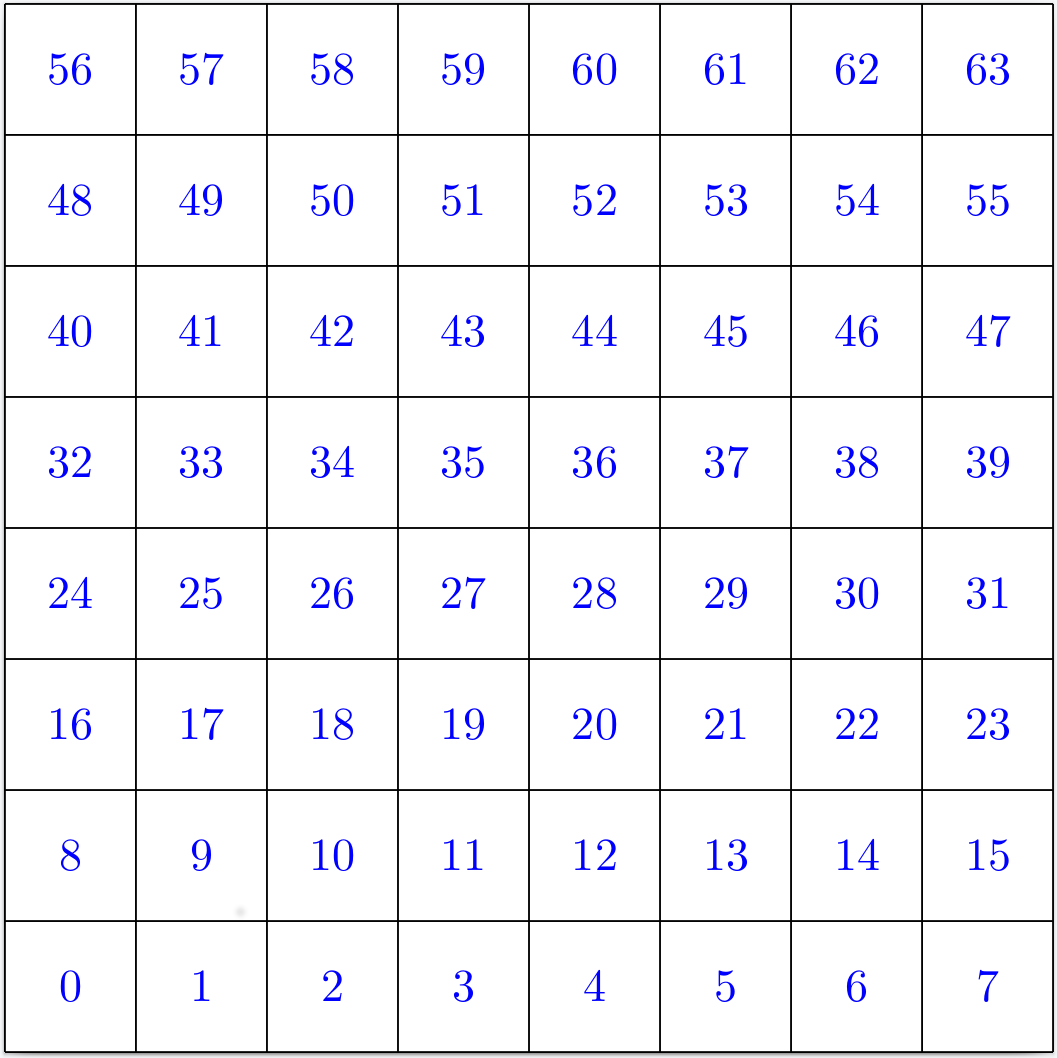
\includegraphics[height=3cm,width=4.5cm]{images/grid8cm.png}
\end{center}

The code for this is:

\vspace{1em}
\begin{tcblisting}{%
        title={\bfseries\sffamily Placing a Picture at an Arbitrary Location},
        minted language=tex,
        listing only,
        minted options={autogobble,escapeinside=``}}
        The  most straightforward  one  is to simply not  create  a \verb|figure|  or
        \verb|table| environment and  put a picture or table  right where you want it 
        in the text:

        \begin{center}
            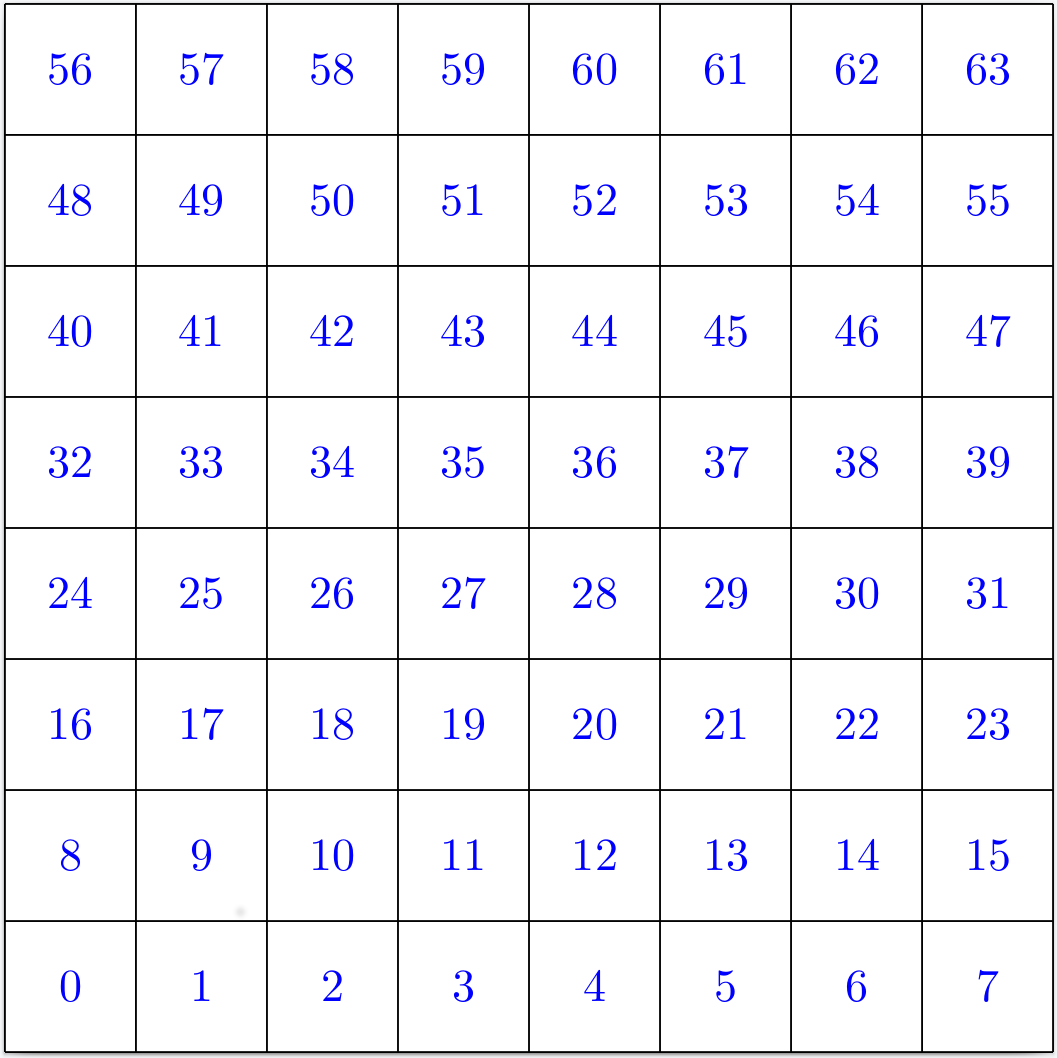
\includegraphics[height=3cm,width=4.5cm]{images/grid8cm.png}
        \end{center}

        the code for this is:
\end{tcblisting}
\vspace{1em}

The \mintinline{tex}{\begin{center}...\end{center}} is of course optional.

You can even place  a picture in the middle of text like  it were text itself,
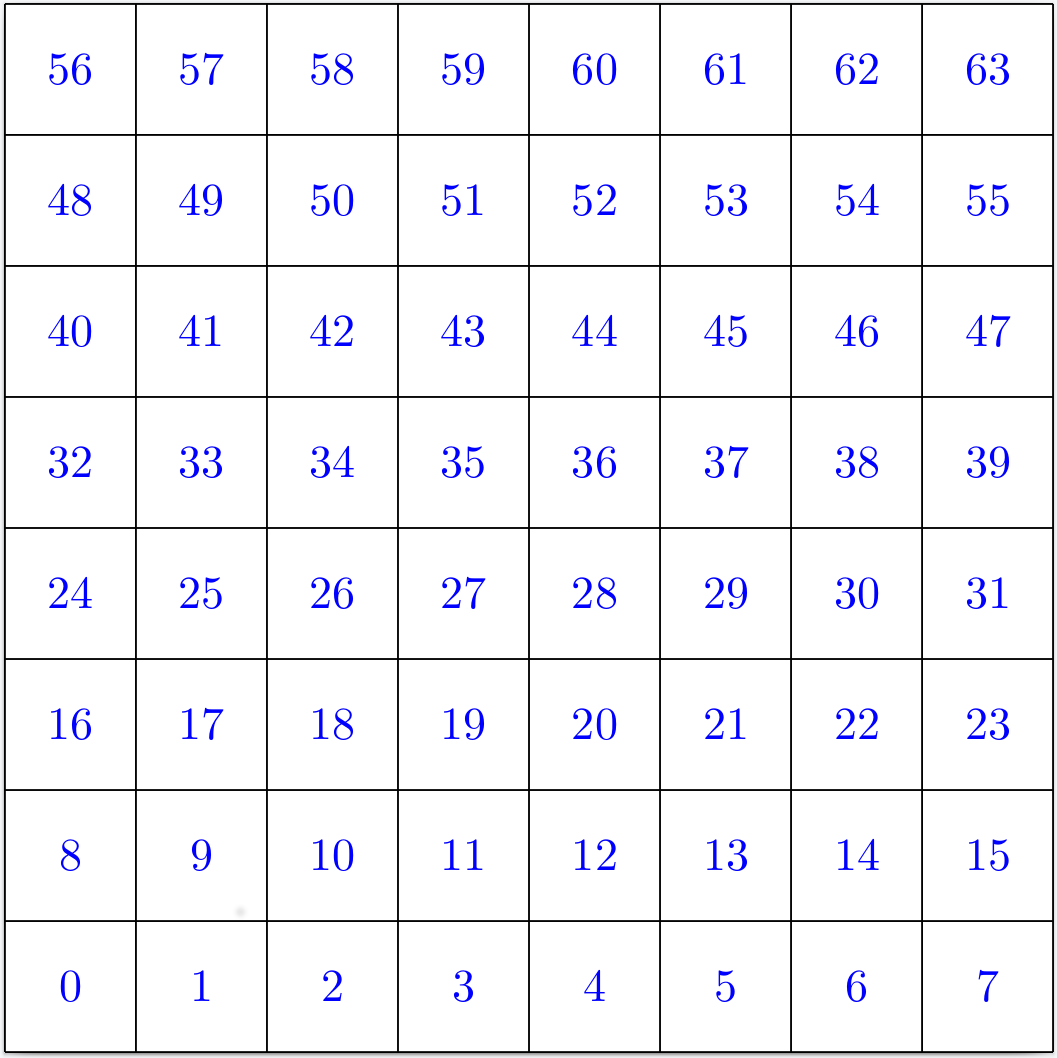
\includegraphics[height=2em,width=4em]{images/grid8cm.png}   as   demonstrated
here. Though this is admittedly rarely a sensible solution.

\vspace{1em}
\begin{tcblisting}{%
        title={\bfseries\sffamily Placing a Picture inside Text},
        minted language=tex,
        listing only,
        minted options={autogobble,escapeinside=``}}

    You can even place a picture in the middle of text like it were text itself,
    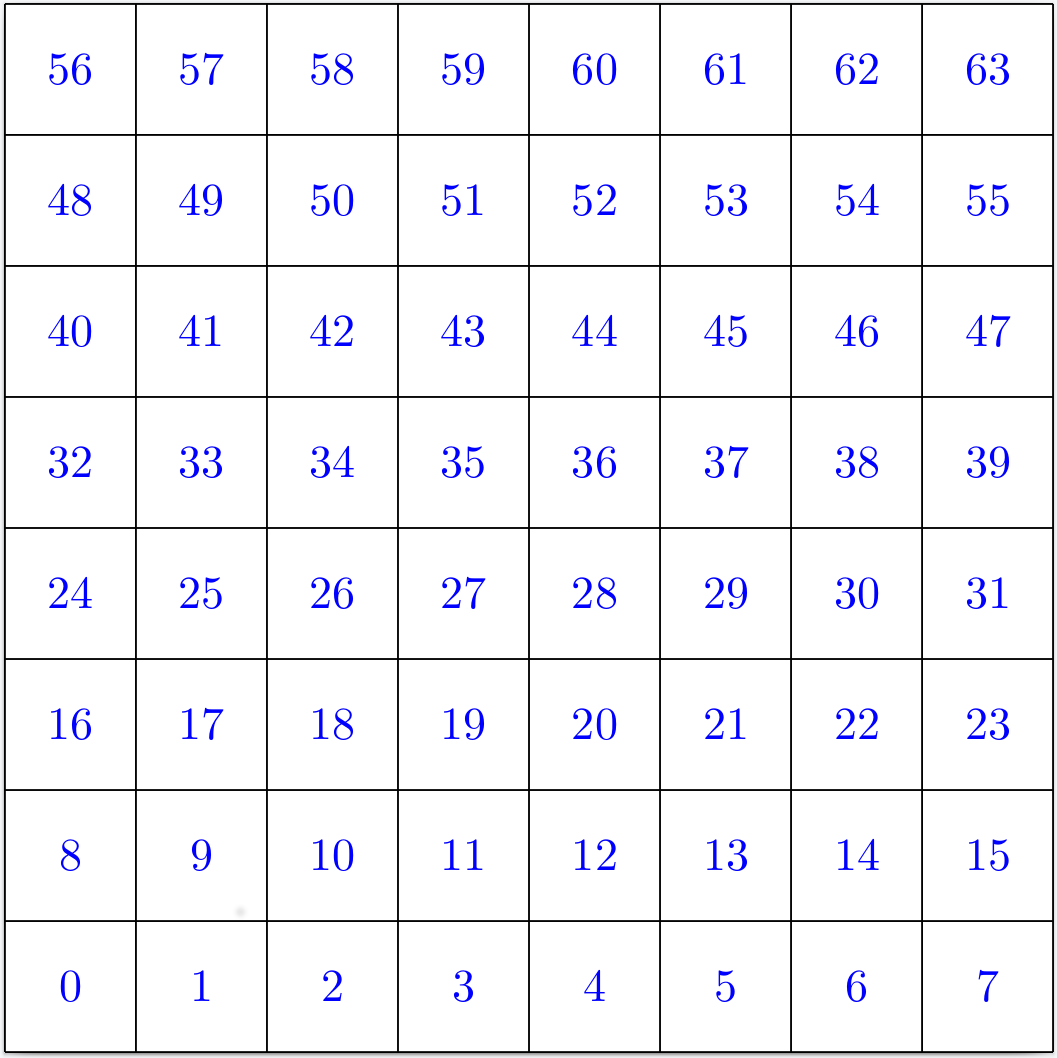
\includegraphics[height=2em,width=4em]{images/grid8cm.png}  as  demonstrated
    here. Though this is admittedly rarely a sensible solution.
\end{tcblisting}
\vspace{1em}

The same goes for tabular environments:

\begin{center}
    \begin{tabular}{ll}
        \toprule
        a & a \\
        a & a \\
        \bottomrule
    \end{tabular}
\end{center}

\vspace{1em}
\begin{tcblisting}{%
        title={\bfseries\sffamily Placing a Tabular at an Arbitrary Location},
        minted language=tex,
        listing only,
        minted options={autogobble,escapeinside=``}}
    The same goes for tabular environments:

    \begin{center}
        \begin{tabular}{ll}
            \toprule
            a & a \\
            a & a \\
            \bottomrule
        \end{tabular}
    \end{center}
\end{tcblisting}
\vspace{1em}

If we want to get very silly indeed, we can even do the same trick with tables
and put them somewhere in  the middle of our text: \begin{tabular}{ll}\toprule
a & a \\a & a\\\bottomrule\end{tabular}. Though really, do not do this.

\vspace{1em}
\begin{tcblisting}{%
        title={\bfseries\sffamily Placing a Tabular inside Text},
        minted language=tex,
        listing only,
        minted options={autogobble,escapeinside=``}}

    If  we want to  get very  silly indeed,  we can  even do the  same trick with 
    tables and put them somewhere in the  middle of our text: \begin{tabular}{ll}
    \toprule a & a \\ a & a\\\bottomrule\end{tabular}.  Though  really, do not do 
    this.
\end{tcblisting}
\vspace{1em}

As you have undoubtedly noticed, there  are no captions for these pictures and
tables. Often, in such cases, they  are indeed not needed. Float numbers allow
an author  to refer  to a  float and a  reader to  find it. Captions  allow to
understand the  float without having  to have  the corresponding main  body of
text right  besides it. So when we  insert a picture  or a table and  place it
right where we want it, it does not necessarily make sense to give it a number
and a caption, because the information needed to understand the content of the
inserted element  is right there. Or at  least it should be. Referring  to the
picture, table or other content via a  caption and numberic index would be odd
and cumbersome in this situation.


% -------------------------------------------------------------------------- %
\section{Captions Outside Floats}
\label{sec:captions-outside-floats}
% -------------------------------------------------------------------------- %

With that  said, we  still sometimes  want to  have numbers  and captions. For
example,  I recently  wrote a  report where  the maximum  number of  pages was
limited.   In order  to  tweak  my document  to  utilize  that limited  number
of  pages  to  their  optimum,  \LaTeX's floating  mechanisms  just  were  not
suitable. However,  I still  wanted  to have  the  basic look  and  feel of  a
document which  was using floats;  the reader was  not supposed to  notice any
difference. I carefully sized  and placed my pseudo-floats  at the appropriate
locations to best utilize the limited page space.

Doing this requires solving two problems:

\begin{itemize}\firmlist
    \item How do we create captions outside of floating environments?
    \item How  do we  keep the captions  and the content  to which  they refer
        associated so that they are not split over page breaks?
\end{itemize}

As always in \LaTeX, there are many  ways to achieve this. I will present four
answers to the first question, and one solution for the second problem.

Having  captions  oustide of  floats  can  be  achieved, among  other  things,
wich the \pacname{caption},  \pacname{capt-of} and \pacname{captdef} packages.
The  packages  \pacname{caption}  and   \pacname{capt-of}  provide  a  command
\verb|\captionof|, whereas you  can define your own commands for  each type of
float in the \pacname{captdef} package.

\begin{tcblisting}{%
        title={\bfseries\sffamily Non-Float Captions with the \texttt{capt-of} or \texttt{caption} Packages},
        minted language=tex,
        listing only,
        minted options={autogobble,escapeinside=``}}
        \includegraphics[width=0.5\textwidth]{images/bestPictureEver.jpeg}
        \captionof{figure}{This is a figure caption outside a float.}
\end{tcblisting}

\begin{tcblisting}{%
        title={\bfseries\sffamily Non-Float Captions with the \texttt{captdef} Package},
        minted language=tex,
        listing only,
        minted options={autogobble,escapeinside=``}}
        % Syntax: \DeclareCaption{command}{counter}:
        \DeclareCaption{\figcaption}{figure}
        \DeclareCaption{\tabcaption}{table}
        \includegraphics[width=0.5\textwidth]{images/bestPictureEver.jpeg}
        \figcaption{This is a figure caption outside a float.}
\end{tcblisting}


If you are using the \pacname{memoir}  document class (such as this document),
you  have a  similar  mechanism  available as  offered  by the  \verb|captdef|
package, with additional formatting options:

\begin{tcblisting}{%
        title={\bfseries\sffamily Defining a Non-Float Caption in \texttt{memoir}},
        minted language=tex,
        listing only,
        minted options={autogobble,escapeinside=||}}
        % Preamble
        \newfixedcaption{\figcaption}{figure}
        \newfixedcaption{\tabcaption}{table}
        \captiontitlefont{\small}
        \captionnamefont{\bfseries\small}
        \captiondelim{: }
        |\ldots|
        \begin{document}
        |\ldots|
        \includegraphics[width=0.5\textwidth]{images/bestPictureEver.jpeg}
        \figcaption{This is a figure caption outside a float.}
        |\ldots|
\end{tcblisting}

For more information, consult the documentation of the respective packages.


For creating an unbreakable  unit of caption and content, I  usually go with a
minipage. There are quite a  lot of other types of boxes  in \TeX\ and \LaTeX,
but in my experience, minipages have proven most robust for this purpose.


\begin{tcblisting}{%
        title={\bfseries\sffamily Using a Minipage to Keep Caption and Content Together},
        minted language=tex,
        %listing only,
        minted options={autogobble,escapeinside=||}}
    \begin{minipage}{\textwidth}
        \centering
        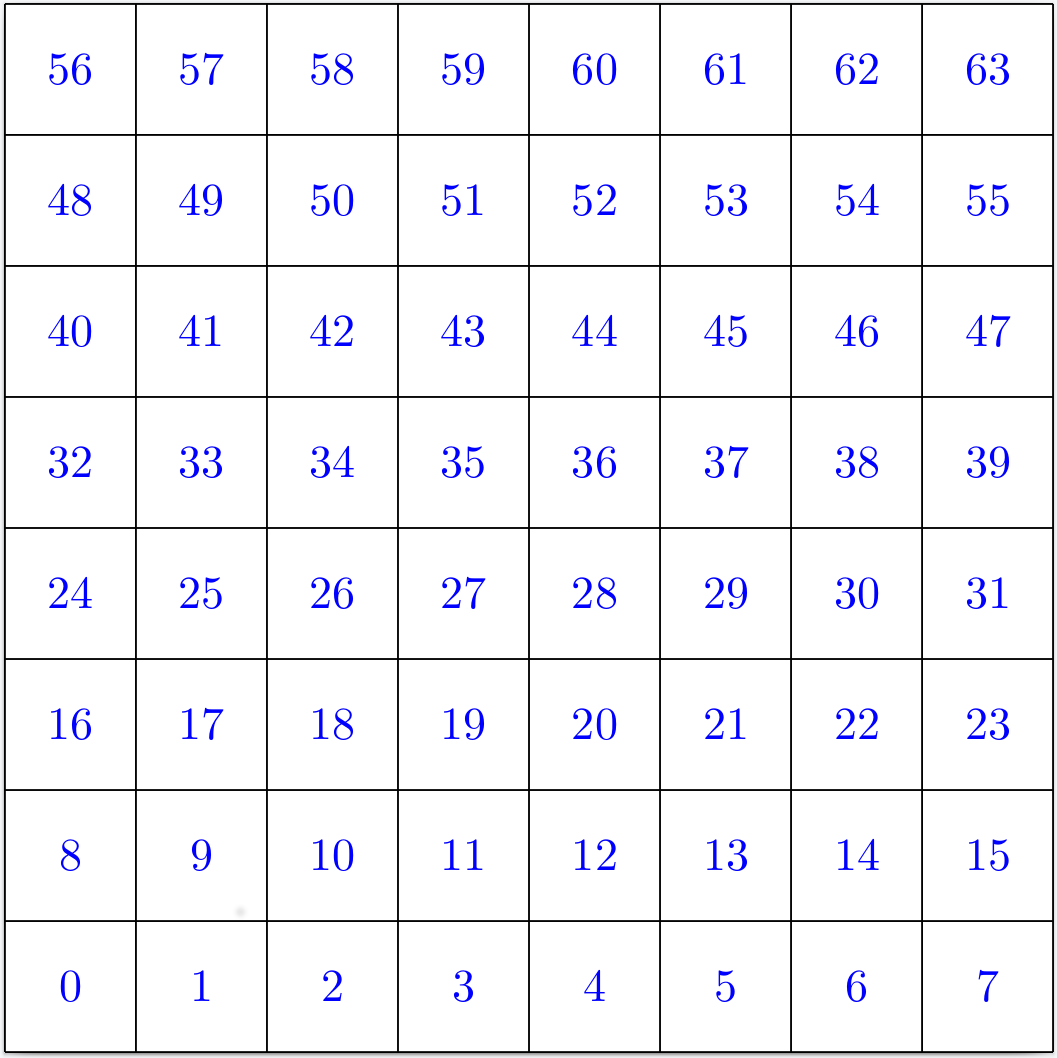
\includegraphics[width=6cm]{images/grid8cm.png}
        \figcaption{A numbered grid}
    \end{minipage}
\end{tcblisting}

If one were to feel so inclined, one could define a new environment with this
or similar code, of course.


% -------------------------------------------------------------------------- %
\section{A Tiny Issue}
\label{sec:issue}
% -------------------------------------------------------------------------- %

This section  has been inspired by  the manuals for the  \pacname{captdef} and
\pacname{capt-of}   packages  \cite{ctan:package:capt-of,ctan:package:captdef}
and appears practically identically in those.

There  is  one  potential  problem  with  using  captions  in  a  non-floating
context: The commands which are used  for the standalone captions increase the
respective content  type's counter  (figure, table, etc.). When  mixing floats
and non-floats of the same type, for example like so:

\begin{tcblisting}{%
        title={\bfseries\sffamily Mixing Floats and Non-Floats},
        minted language=tex,
        listing only,
        minted options={autogobble,escapeinside=||}}

        <text>

        \begin{figure}
            \includegraphics{magnificent-picture.png}
            \caption{A magnificent picture!}
        \end{figure}

        <more text>

        \includegraphics{another-nice-picture.png}
        \figcaption{A nice picture!}

        <yet more text>
\end{tcblisting}

If the \code{figure} does not fit anywhere between where it is in the text and
where the non-floating image is included, it can float after the second image,
resulting in the figure numbers getting out of order:

\begin{tcblisting}{%
        title={\bfseries\sffamily Mixing Floats and Non-Floats, Figure Numbers Out of Order},
        minted language=tex,
        listing only,
        minted options={autogobble,escapeinside=||}}
        <text>
        <Figure [n + 1]> % A nice picture!
        <more text>
        <Figure [n]>     % A magnificent picture!
        <yet more text>
\end{tcblisting}

When using only floats (or only non-floats) this cannot happen, because as per
the  rules laid  out  in Section~\label{chap:jinxed},  a  float which  appears
before another float in  the source code can never appear  after that float in
the result. This  is also one  potential advantage  of sticking to  floats and
using an  \code{H} parameter, for  example via the  \pacname{floatrow} package
(at least as far as I'm aware).

The bottom line  is this: Once you take control over  where content is placed,
beware of dragons.

% ========================================================================== %
\begin{thebibliography}{1}
\label{bibliography}
% ========================================================================== %

    \bibitem{lamport}
        Leslie Lamport, Digital Equipment Corporation.
        ``\emph{\LaTeX{} -- A Document Preparation System}'',
        2nd Edition,
        1994,
        Addison-Wesley Publishing Company.

    \bibitem{mori:tables}
        Lapo Mori,
        ``\emph{Tables in \LaTeXe: Packages and Methods}'',
        The Prac\TeX{} Journal,
        2007-FEB-20.
        [Online],
        \href{https://www.tug.org/pracjourn/2007-1/mori/mori.pdf}
             {\nolinkurl{https://www.tug.org/pracjourn/2007-1/mori/mori.pdf}},
        [Accessed: 2017-MAR-27].

    \bibitem{ctan:package:caption}
        Axel Sommerfeldt.
        ``\emph{Package caption -- Customising captions in floating environments}'',
        Version 2016-05-22,
        2016-MAY-22.
        [Online],
        \href{http://ctan.org/pkg/caption}{\nolinkurl{http://ctan.org/pkg/caption}},
        [Accessed: 2017-MAR-26].

    \bibitem{ctan:topic:caption}
        Comprehensive \TeX{} Archive Network.
        ``\emph{Topic caption}''.
        [Online],
        \href{http://ctan.org/topic/caption}{\nolinkurl{http://ctan.org/topic/caption}},
        [Accessed: 2017-MAR-26].

    \bibitem{stackexch:center-centering}
        Enrico Gregorio,
        ``\emph{When should we use \texttt{\textbackslash{}begin\{center\}} 
        instead of \texttt{\textbackslash{}centering?}}'',
        [Online],
        \href{http://tex.stackexchange.com/a/23653}
             {\nolinkurl{http://tex.stackexchange.com/a/23653}},
        [Accessed: 2017-MAR-26].
    
    \bibitem{texblog:center-centering}
        stefan,
        ``\emph{\TeX{}Blog -- center vs. centering}''.
        [Online],
        \href{http://texblog.net/latex-archive/floats/center-centering/}
             {\nolinkurl{http://texblog.net/latex-archive/floats/center-centering/}},
        [Accessed: 2017-MAR-27].

    \bibitem{stackesch:h-ht}
        Stefan Kottwitz,
        ``\emph{h float specifier changed to ht warning when not attempting to specify a float}''.
        [Online],
        \href{http://tex.stackexchange.com/a/1527}
             {\nolinkurl{http://tex.stackexchange.com/a/1527}},
        [Accessed: 2017-MAR-27].

    \bibitem{ctan:package:floatrow}
        Olga Lapko.
        ``\emph{floatrow -- Modifying the layout of floats}'',
        Version 0.3b,
        2009-AUG-02.
        [Online],
        \href{http://ctan.org/pkg/float}{\nolinkurl{http://ctan.org/pkg/float}},
        [Accessed: 2017-MAR-27].

    \bibitem{ctan:package:float}
        Anselm Lingnau.
        ``\emph{float -- Improved interface for floating objects}'',
        Version 1.3d,
        2001-NOV-08.
        [Online],
        \href{http://ctan.org/pkg/float}{\nolinkurl{http://ctan.org/pkg/float}},
        [Accessed: 2017-MAR-27].

    \bibitem{ctan:package:capt-of}
        Robin Fairbairns.
        ``\emph{Capt-of -- Captions on more than floats}'',
        2010-JAN-22.
        [Online],
        \href{https://www.ctan.org/pkg/capt-of}
             {\nolinkurl{https://www.ctan.org/pkg/capt-of}},
        [Accessed: 2017-MAR-28].

    \bibitem{ctan:package:captdef}
        Robin Fairbairns.
        ``\emph{Captdef -- Declare free-standing \code{\textbackslash{}caption} commands}'',
        2010-MAR-06.
        [Online],
        \href{https://www.ctan.org/pkg/captdef}
             {\nolinkurl{https://www.ctan.org/pkg/captdef}},
        [Accessed: 2017-MAR-28].

\end{thebibliography}

\end{document}
